\documentclass[11pt,letterpaper]{article}

\usepackage[margin=0.88in,top=0.86in,bottom=0.86in]{geometry}
\usepackage[utf8]{inputenc}
\usepackage[T1]{fontenc}
\usepackage{newpxtext,newpxmath} % Palatino typography
\usepackage{microtype}
\usepackage{amsmath,amsfonts}
\usepackage{graphicx}
\usepackage{booktabs}
\usepackage{xcolor}
\usepackage{fancyhdr}
\usepackage{enumitem}
\usepackage{titlesec}
\usepackage{tikz}
\usetikzlibrary{shapes.geometric,arrows.meta,positioning,calc,decorations.pathmorphing}
\usepackage{listings}
\usepackage{hyperref}

% Palette
\definecolor{primaryblue}{RGB}{2, 100, 160}
\definecolor{accentindigo}{RGB}{60, 50, 190}
\definecolor{accentteal}{RGB}{12, 110, 105}
\definecolor{darkslate}{RGB}{28, 38, 52}
\definecolor{warmbg}{RGB}{252, 250, 247}
\definecolor{boxborder}{RGB}{210, 220, 230}
\definecolor{calloutbg}{RGB}{242, 248, 255}
\definecolor{codebg}{RGB}{247, 249, 252}
\definecolor{codeframe}{RGB}{220, 228, 238}

% Hyperref
\hypersetup{
    colorlinks=true,
    linkcolor=accentindigo,
    citecolor=primaryblue,
    urlcolor=accentteal
}

% Section Titles - Strict colon-free heading rule
\titleformat{\section}{\Large\bfseries\color{primaryblue}}{\thesection.}{0.6em}{}[\vspace{-0.3em}{\color{boxborder}\hrule height 0.7pt}]
\titleformat{\subsection}{\large\bfseries\color{accentindigo}}{\thesubsection}{0.6em}{}
\titleformat{\subsubsection}{\normalsize\bfseries\color{darkslate}}{\thesubsubsection}{0.6em}{}
\titlespacing*{\section}{0pt}{5pt plus 1.5pt minus 1pt}{2.5pt plus 1pt minus 1pt}
\titlespacing*{\subsection}{0pt}{3.5pt plus 1pt minus 1pt}{1.5pt plus 1pt minus 1pt}
\setlength{\textfloatsep}{7pt plus 1.5pt minus 1.5pt}
\setlength{\intextsep}{6pt plus 1.5pt minus 1.5pt}
\setlength{\floatsep}{6pt plus 1.5pt minus 1.5pt}
\setlength{\abovedisplayskip}{3.5pt plus 1pt minus 1pt}
\setlength{\belowdisplayskip}{3.5pt plus 1pt minus 1pt}
\setlength{\abovedisplayshortskip}{2pt plus 1pt minus 1pt}
\setlength{\belowdisplayshortskip}{2pt plus 1pt minus 1pt}

% Headers / Footers
\pagestyle{fancy}
\fancyhf{}
\fancyhead[L]{\small\sffamily\color{darkslate}\textbf{Cultural Mechanics}}
\fancyhead[R]{\small\sffamily\color{primaryblue}\textbf{Lecture 05}}
\fancyfoot[L]{\scriptsize\sffamily\color{darkslate!60}Semantic Mechanics Project $\cdot$ Mathematical Linguistics Group}
\fancyfoot[R]{\small\sffamily\color{darkslate}\thepage}
\renewcommand{\headrulewidth}{0.4pt}
\renewcommand{\footrulewidth}{0.4pt}

% Callout Boxes
\newcommand{\calloutbox}[2]{%
\vspace{0.3em}\noindent
\begin{tikzpicture}
\node[draw=primaryblue, fill=calloutbg, rounded corners=4pt, line width=0.9pt, text width=\dimexpr\linewidth-20pt\relax, inner sep=6.5pt] {
    {\sffamily\bfseries\color{primaryblue}#1}\par\vspace{0.2em}{\color{boxborder}\hrule height 0.5pt}\vspace{0.35em}
    {\small\color{darkslate}#2}
};
\end{tikzpicture}\vspace{0.3em}
}

\newcommand{\socraticbox}[2]{%
\vspace{0.3em}\noindent
\begin{tikzpicture}
\node[draw=accentindigo, fill=warmbg, rounded corners=4pt, line width=0.9pt, text width=\dimexpr\linewidth-20pt\relax, inner sep=6.5pt] {
    {\sffamily\bfseries\color{accentindigo}#1}\par\vspace{0.2em}{\color{boxborder}\hrule height 0.5pt}\vspace{0.35em}
    {\small\color{darkslate}#2}
};
\end{tikzpicture}\vspace{0.3em}
}

% Code Listings
\lstset{
    backgroundcolor=\color{codebg},
    frame=single,
    rulecolor=\color{codeframe},
    basicstyle=\ttfamily\scriptsize,
    keywordstyle=\color{primaryblue}\bfseries,
    commentstyle=\color{accentteal}\itshape,
    stringstyle=\color{accentindigo},
    numbers=none,
    breaklines=true,
    showstringspaces=false,
    tabsize=2,
    xleftmargin=6pt,
    xrightmargin=6pt
}

\begin{document}

% Title Block
\begin{center}
    {\small\sffamily\bfseries\color{darkslate} SEMANTIC MECHANICS PROJECT $\cdot$ MATHEMATICAL LINGUISTICS GROUP}\\[0.7em]
    {\LARGE\bfseries\color{primaryblue} Lecture 05: Cognitive Translation}\\[0.35em]
    {\Large\bfseries\color{primaryblue} Neurobiological Manifolds, Modality Projection, and Channel Thermodynamics}\\[0.4em]
    {\normalsize\sffamily\color{darkslate} \textbf{Course:} Cultural Mechanics $\cdot$ \textbf{Semester:} Autumn 2026}\\[0.25em]
    {\small\sffamily\color{darkslate!80} \textbf{Prerequisites:} Dynamical Systems, Rate-Distortion Theory, Differential Geometry, Non-Equilibrium Thermodynamics}\\[0.25em]
    {\small\sffamily\color{darkslate!80} \textbf{Foundational Readings:} Kuhl (2004), Shannon (1948), Stokoe (1960), Cover \& Thomas (2006), Friston (2010)}
\end{center}
\vspace{0.1em}
\hrule height 1.2pt \vspace{0.7em}

\section{Multilingual Manifolds and Attractor Dynamics}

Welcome to \textit{Lecture 05: Cognitive Translation}. In Lecture 03, we formalized the differential geometry and category-theoretic invariants of translation, establishing continuous manifold mappings and adjoint functors. In Lecture 04, we derived the non-equilibrium thermodynamics of physical sequence transformation, bounding the entropic dissipation of typographic work. We now conclude the \textbf{Translation Trilogy} by investigating how physical nervous systems, assistive technologies, and multi-modal human bodies execute translation across fundamentally disparate cognitive substrates.

Translation is not solely an algorithmic mapping between symbolic strings; it is an embodied thermodynamic and neurocomputational act. Whether routing conceptual representations between competing phonetic attractor basins in a polyglot cortex, compressing intentional semantics through severely bandlimited motor channels in augmentative communication, or projecting high-dimensional spatio-temporal sign language onto sequential acoustic waveforms, cognitive translation requires physical energy, sensory arbitration, and continuous error minimization.

\subsection{Native Language Attunement as Potential Energy Wells}
During infancy, human neural auditory circuits undergo developmental perceptual narrowing. The unconstrained phonetic space of human vocality $\mathcal{V} \subset \mathbb{R}^d$ collapses into discrete phonetic categories governed by the native language $\mathcal{L}_1$. From the perspective of dynamical systems, native language acquisition represents the stabilization of deep \textbf{potential energy attractor wells} on a cognitive neural manifold $\mathcal{M}$.

Let $\mathbf{x}(t) \in \mathcal{M}$ represent the time-dependent state of a cortical linguistic network. The continuous neural trajectory evolves under gradient descent upon a non-convex free-energy potential $U(\mathbf{x}; \boldsymbol{\theta})$ perturbed by stochastic cognitive fluctuations:
\begin{equation}
\frac{d\mathbf{x}}{dt} = -\nabla U(\mathbf{x}; \boldsymbol{\theta}) + \sqrt{2 D}\, \boldsymbol{\xi}(t)
\end{equation}
where $\boldsymbol{\theta}$ denotes synaptic connection weights, $D$ is the neural diffusion coefficient, and $\boldsymbol{\xi}(t)$ is Gaussian white noise satisfying $\langle \boldsymbol{\xi}(t) \boldsymbol{\xi}(t^\prime)^\top \rangle = \mathbf{I} \delta(t - t^\prime)$. 

In an infant before perceptual narrowing ($t < t_{\text{critical}}$), the potential $U(\mathbf{x})$ is approximately flat, permitting flexible discrimination of all cross-linguistic phonetic contrasts. Through continuous sensory exposure to $\mathcal{L}_1$, synaptic plasticity deepens local potential minima corresponding to native phonemes and grammatical templates:
\begin{equation}
U_{\mathcal{L}_1}(\mathbf{x}) = -\sum_{i=1}^{M_1} A_i \exp\left( -\frac{\|\mathbf{x} - \mathbf{c}_i\|^2}{2\sigma_i^2} \right)
\end{equation}
where $\mathbf{c}_i \in \mathcal{M}$ denotes the attractor center of phoneme $i$, $A_i > 0$ is the well depth, and $\sigma_i$ is the receptive field width.

\subsection{Second-Language Acquisition and Potential Barrier Transport}
When an adult learner acquires a second language $\mathcal{L}_2$, the existing $\mathcal{L}_1$ attractor wells exert severe gravitational interference. An incoming auditory token $\mathbf{y} \in \mathcal{L}_2$ falling near an $\mathcal{L}_1$ well is inexorably pulled into the native attractor, explaining the physical basis of native phonetic perceptual assimilation.

Establishing distinct $\mathcal{L}_2$ representations requires modifying the underlying potential landscape to construct new attractors $\mathbf{c}_j^{\prime} \in \mathcal{L}_2$. The cognitive transport cost of translating an intent from $\mathcal{L}_1$ to $\mathcal{L}_2$ corresponds to the \textbf{Kramers escape rate} across the potential barrier $\Delta U = U(\mathbf{x}^\ddagger) - U(\mathbf{c}_i)$:
\begin{equation}
r_{\text{switch}} = \frac{\sqrt{|U^{\prime\prime}(\mathbf{c}_i) U^{\prime\prime}(\mathbf{x}^\ddagger)|}}{2\pi \gamma} \exp\left( -\frac{\Delta U}{k_B T_{\text{eff}}} \right)
\end{equation}
where $\mathbf{x}^\ddagger$ is the saddle point separating the two language basins, $\gamma$ is neural damping, and $T_{\text{eff}}$ represents metabolic arousal or attentional temperature. In novice bilinguals, $\Delta U$ is large, resulting in slow, conscious lexical translation and measurable cognitive latency ($\sim 200$--$400\text{ ms}$).

\begin{figure}[htbp]
\centering
\resizebox{0.95\linewidth}{!}{%
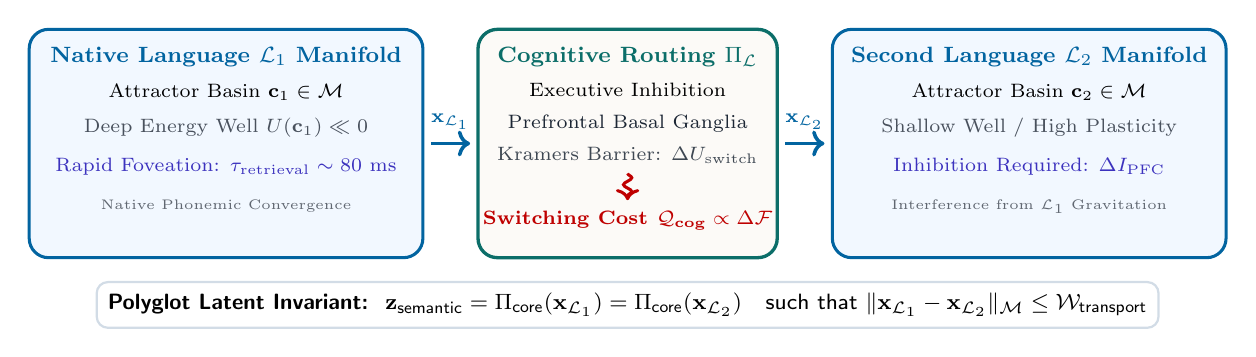
\begin{tikzpicture}[every node/.style={font=\sffamily}]
    % Language 1 Basin
    \draw[fill=calloutbg, draw=primaryblue, line width=1.1pt, rounded corners=7pt] (-7.6,-1.45) rectangle (-2.6,1.45);
    \node[color=primaryblue, font=\bfseries\footnotesize] at (-5.1, 1.10) {Native Language $\mathcal{L}_1$ Manifold};
    \node[font=\scriptsize] at (-5.1, 0.65) {Attractor Basin $\mathbf{c}_1 \in \mathcal{M}$};
    \node[font=\scriptsize, color=darkslate!80] at (-5.1, 0.20) {Deep Energy Well $U(\mathbf{c}_1) \ll 0$};
    \node[font=\scriptsize, color=accentindigo] at (-5.1, -0.30) {Rapid Foveation: $\tau_{\text{retrieval}} \sim 80\text{ ms}$};
    \node[font=\tiny, color=darkslate!70] at (-5.1, -0.80) {Native Phonemic Convergence};

    % Cognitive Routing Engine
    \draw[fill=warmbg, draw=accentteal, line width=1.2pt, rounded corners=7pt] (-1.9,-1.45) rectangle (1.9,1.45);
    \node[color=accentteal, font=\bfseries\footnotesize] at (0, 1.10) {Cognitive Routing $\Pi_{\mathcal{L}}$};
    \node[font=\scriptsize] at (0, 0.68) {Executive Inhibition};
    \node[font=\scriptsize, color=darkslate] at (0, 0.25) {Prefrontal Basal Ganglia};
    \node[font=\scriptsize, color=darkslate!85] at (0, -0.15) {Kramers Barrier: $\Delta U_{\text{switch}}$};
    \draw[->, line width=1.1pt, color=red!75!black, decorate, decoration={snake, amplitude=1.5pt, segment length=5pt}] (0, -0.38) -- (0, -0.72);
    \node[font=\scriptsize\bfseries, color=red!75!black] at (0, -0.98) {Switching Cost $\mathcal{Q}_{\text{cog}} \propto \Delta \mathcal{F}$};

    % Transition Vectors
    \draw[->, line width=1.3pt, color=primaryblue] (-2.5, 0.0) -- (-2.0, 0.0) node[midway, above=1pt, font=\scriptsize\bfseries] {$\mathbf{x}_{\mathcal{L}_1}$};
    \draw[->, line width=1.3pt, color=primaryblue] (2.0, 0.0) -- (2.5, 0.0) node[midway, above=1pt, font=\scriptsize\bfseries] {$\mathbf{x}_{\mathcal{L}_2}$};

    % Language 2 Basin
    \draw[fill=calloutbg, draw=primaryblue, line width=1.1pt, rounded corners=7pt] (2.6,-1.45) rectangle (7.6,1.45);
    \node[color=primaryblue, font=\bfseries\footnotesize] at (5.1, 1.10) {Second Language $\mathcal{L}_2$ Manifold};
    \node[font=\scriptsize] at (5.1, 0.65) {Attractor Basin $\mathbf{c}_2 \in \mathcal{M}$};
    \node[font=\scriptsize, color=darkslate!80] at (5.1, 0.20) {Shallow Well / High Plasticity};
    \node[font=\scriptsize, color=accentindigo] at (5.1, -0.30) {Inhibition Required: $\Delta I_{\text{PFC}}$};
    \node[font=\tiny, color=darkslate!70] at (5.1, -0.80) {Interference from $\mathcal{L}_1$ Gravitation};

    % Lower Invariant Box
    \node[draw=boxborder, fill=white, rounded corners=4pt, line width=0.8pt, inner sep=4pt] at (0,-2.05) {
        \footnotesize\textbf{Polyglot Latent Invariant:}\; $\mathbf{z}_{\text{semantic}} = \Pi_{\text{core}}(\mathbf{x}_{\mathcal{L}_1}) = \Pi_{\text{core}}(\mathbf{x}_{\mathcal{L}_2}) \quad \text{such that } \|\mathbf{x}_{\mathcal{L}_1} - \mathbf{x}_{\mathcal{L}_2}\|_{\mathcal{M}} \le \mathcal{W}_{\text{transport}}$
    };
\end{tikzpicture}%
}
\caption{Dynamical Landscape of Multilingual Cognitive Translation: neural representations occupy language-specific attractor basins on a shared cortical manifold $\mathcal{M}$. Translating between languages requires prefrontal executive control to cross potential energy barriers $\Delta U$, dissipating cognitive metabolic work.}
\label{fig:multilingual_dynamics}
\end{figure}

\subsection{Polyglot Neural Geometries and Semantic Latent Invariance}
In hyperpolyglots (individuals fluent in $>6$ languages), neuroimaging demonstrates that cortical activation does not linearly expand with the number of languages. Rather, polyglot neural architecture establishes a \textbf{language-invariant semantic core manifold} $\mathcal{Z}_{\text{core}}$, coupled to peripheral language-specific projection operators:
\begin{equation}
\mathbf{s}_k = \mathbf{W}_k \mathbf{z}_{\text{core}} + \mathbf{b}_k, \qquad k \in \{1, 2, \dots, K\}
\end{equation}
where $\mathbf{z}_{\text{core}} \in \mathcal{Z}_{\text{core}}$ encodes conceptual propositions independent of phonology, and $\mathbf{W}_k$ projects into the phonetic-syntactic realization space of language $k$.

Because the latent core $\mathbf{z}_{\text{core}}$ is shared, translation between any language pair $(\mathcal{L}_a, \mathcal{L}_b)$ is achieved through the algebraic composition:
\begin{equation}
\tau_{a \to b}(\mathbf{s}_a) = \mathbf{W}_b \mathbf{W}_a^+ \mathbf{s}_a
\end{equation}
where $\mathbf{W}_a^+$ is the Moore-Penrose pseudoinverse. The thermodynamic cost of polyglot translation is thus bounded not by language count, but by the condition number $\kappa(\mathbf{W}_a) = \|\mathbf{W}_a\| \|\mathbf{W}_a^+\|$ of the source projection operator.

\section{Augmentative Communication and Motor Bottlenecks}

\subsection{Information Transmission under Extreme Channel Constraints}
While normative vocal speech achieves an output bandwidth of $35$--$50\text{ bits/second}$ ($\sim 150\text{ words/minute}$), individuals with severe physical neuro-motor impairments (e.g., amyotrophic lateral sclerosis, high-level cervical spinal cord injury, dyskinetic cerebral palsy) lose somatic voluntary control over the $100+$ vocal tract muscles.

Communication must be mediated by **Augmentative and Alternative Communication (AAC)** interfaces utilizing minimal residual physiological degrees of freedom:
\begin{itemize}[noitemsep,topsep=1.5pt]
    \item \textbf{Eye-Gaze Tracking:} Ocular saccades and sustained fixations measured via infrared pupil-corneal reflection.
    \item \textbf{Single-Switch Mechanical Scanning:} Binary temporal closures executed by a single finger, cheek twitch, or head switch.
    \item \textbf{Electromyographic / Brain-Computer Interfaces (BCIs):} Sub-threshold motor unit action potentials or cortical electrocorticographic (ECoG) sensorimotor rhythms.
\end{itemize}

\subsection{Rate-Distortion and Selection Dynamics}
In AAC systems, each discrete symbol selection requires an unavoidable physical latency $T_{\text{selection}}$. In an eye-tracking virtual keyboard, intentional selection requires a **dwell time** $T_{\text{dwell}} \approx 300$--$600\text{ ms}$ to disambiguate deliberate communicative fixation from natural perceptual saccades (the "Midas Touch" problem).

In single-switch scanning, symbols are arranged in a matrix of size $R \times C$. A highlight cursor scans sequentially across rows at period $\tau_{\text{scan}} \approx 500\text{ ms}$. Selecting a target character at position $(r, c)$ requires an expected time:
\begin{equation}
\mathbb{E}[T_{\text{selection}}] = \sum_{r=1}^R \sum_{c=1}^C P(r, c) \Big( r \tau_{\text{scan}} + c \tau_{\text{scan}} + 2 T_{\text{reaction}} \Big)
\end{equation}
Consequently, uncompressed character-by-character single-switch selection yields an effective communicative bit rate:
\begin{equation}
\mathcal{R}_{\text{raw}} = \frac{H(\Sigma)}{\mathbb{E}[T_{\text{selection}}]} \approx \frac{4.7\text{ bits}}{4.2\text{ seconds}} \approx 1.12\text{ bits/second} \quad (\sim 3\text{--}5\text{ words/minute})
\end{equation}
This establishes an extreme **information-theoretic channel bottleneck**: human cognitive intent forms at $\sim 40\text{ bits/sec}$, yet the physical motor channel transmits at $\approx 1\text{ bit/sec}$---a $40\times$ communicative impedance mismatch.

\begin{table}[htbp]
\centering
\resizebox{\linewidth}{!}{%
\begin{tabular}{lrrrr}
\toprule
\textbf{Assistive Communication Modality} & \textbf{Effective Bit Rate} & \textbf{Words / Minute} & \textbf{Physical Degrees of Freedom} & \textbf{Error Rate ($P_e$)} \\
\midrule
Normative Vocal Phonation & $35.0$--$50.0\text{ bps}$ & $140$--$180\text{ wpm}$ & $>100\text{ vocal muscles}$ & $< 0.01$ \\
Direct Physical Keyboard Typing & $15.0$--$25.0\text{ bps}$ & $60$--$100\text{ wpm}$ & $10\text{ independent digits}$ & $\sim 0.02$ \\
Eye-Gaze Dwell Typing (Unassisted) & $3.0$--$5.5\text{ bps}$ & $12$--$22\text{ wpm}$ & $2\text{ ocular angles } (\theta, \phi)$ & $\sim 0.05$ \\
Eye-Gaze + Neural Language Model & $8.0$--$14.0\text{ bps}$ & $30$--$55\text{ wpm}$ & $2\text{ ocular angles } (\theta, \phi)$ & $\sim 0.03$ \\
Single-Switch Row-Column Scan & $0.8$--$1.8\text{ bps}$ & $3$--$7\text{ wpm}$ & $1\text{ binary degree of freedom}$ & $\sim 0.08$ \\
Invasive Sensorimotor ECoG BCI & $6.0$--$12.0\text{ bps}$ & $25$--$48\text{ wpm}$ & $64$--$256\text{ neural electrodes}$ & $\sim 0.06$ \\
\bottomrule
\end{tabular}%
}
\caption{Assistive Communication Channel Physics: severe motor impairments collapse physical channel degrees of freedom, throttling information transmission rates by over an order of magnitude unless augmented by predictive language models.}
\label{tab:aac_rates}
\end{table}

\subsection{Predictive Compression and Semantic Compaction}
To bridge this $40\times$ impedance mismatch, modern cognitive engineering deploys mathematical compression at the semiotic interface:

\textbf{1. Autoregressive Predictive Acceleration:} An n-gram or neural language model computes conditional character and word probabilities $P(w_t \mid w_{<t})$. Offering the top $K$ candidates reduces the expected motor actions per word from $L \approx 5.5$ keystrokes to $\bar{K}_{\text{actions}} \approx 1.8$:
\begin{equation}
\mathcal{C}_{\text{savings}} = 1 - \frac{\sum_{t=1}^N \mathcal{A}(s_t)}{\sum_{t=1}^N |s_t|} \approx 0.65\text{--}0.72
\end{equation}

\textbf{2. Semantic Compaction (Minspeak):} Rather than spelling words orthographically, icons with multi-dimensional semantic associations are combined into short multi-icon sequences (length $2$ or $3$). Because an icon matrix of size $M = 84$ yields $84^2 = 7{,}056$ unique two-symbol combinations, a vocabulary exceeding $5{,}000$ core words can be addressed with exactly two physical switch activations per lexical item, eliminating letter-by-letter spelling.

\section{Cross-Modal Syntax and Spatial Topologies}

\subsection{1D Acoustic Serialization versus 4D Spatio-Temporal Manifolds}
Spoken human languages transmit semantic information over an acoustic transmission line. Because the human vocal tract and auditory cochlea operate in the time domain, speech is constrained to **strictly one-dimensional serial transmission**:
\begin{equation}
\mathbf{s}_{\text{spoken}}(t) \in \mathbb{R}^1, \qquad t \in [0, T]
\end{equation}
To express complex hierarchical, non-local semantic relations, spoken languages must invent elaborate linear grammatical devices: syntactic word order, case inflections, auxiliary verbs, and recursive relative clauses.

In contrast, natural sign languages (such as American Sign Language [ASL] or British Sign Language [BSL]) transmit information visually across **three spatial dimensions plus time**:
\begin{equation}
\mathbf{s}_{\text{signed}}(t) = \Big( \mathbf{x}_{\text{dominant}}(t), \, \mathbf{x}_{\text{non-dominant}}(t), \, \mathbf{q}_{\text{facial}}(t), \, \mathbf{h}_{\text{handshape}}(t) \Big) \in \mathbb{R}^3 \times \mathbb{R}^3 \times \mathcal{S}_{\text{face}} \times \mathcal{H}_{\text{config}}
\end{equation}

\subsection{Simultaneous Spatial Indexing and Classifier Predicates}
Sign language grammar exploits this four-dimensional spatio-temporal medium through **simultaneous parallel morphology**:
\begin{itemize}[noitemsep,topsep=1.5pt]
    \item \textbf{Spatial Loci Formulation:} Referents (agents, patients, locations) are established at specific coordinates $\mathbf{r}_i \in \mathbb{R}^3$ in the signing volume before the chest.
    \item \textbf{Directional Vector Verbs:} A verb of transfer (e.g., \texttt{GIVE}, \texttt{INFORM}) moves along a continuous directed trajectory $\gamma: [0, 1] \to \mathbb{R}^3$ directly connecting source locus $\mathbf{r}_{\text{agent}}$ to destination locus $\mathbf{r}_{\text{recipient}}$:
    \begin{equation}
    \gamma(0) = \mathbf{r}_{\text{agent}}, \qquad \gamma(1) = \mathbf{r}_{\text{recipient}}, \qquad \frac{d\gamma}{dt} = \mathbf{v}_{\text{manner}}
    \end{equation}
    Subject, object, verb root, and manner of motion are transmitted in a **single simultaneous motor act** lasting $\sim 300\text{ ms}$, whereas the equivalent vocal sentence requires a sequential string of $5$--$7$ words lasting $\sim 2{,}000\text{ ms}$.
\end{itemize}

Translating between spoken and signed language is mathematically a **fiber bundle projection**:
\begin{equation}
\pi: \mathcal{E}_{\text{spatial}}^{4\text{D}} \to \mathcal{B}_{\text{temporal}}^{1\text{D}}
\end{equation}
The fiber $\mathcal{F} = \pi^{-1}(t)$ contains rich spatial topological relations that must be serialised into flat relational prepositions when translated into spoken English, and vice versa reconstituted into continuous 3D coordinate trajectories when translated into ASL.

\section{Thermodynamics of Communication Channels}

\subsection{Synchronous Face-to-Face Dialogue versus Asynchronous Media}
A complete physical theory of communication must distinguish between two thermodynamic regimes:

\textbf{1. Synchronous Dialogue:} Two communicators share a continuous mutual observation channel with latency $\Delta t < 100\text{ ms}$. Micro-backchannels (gaze shifts, nod dynamics, paralinguistic murmurs) allow continuous real-time error correction:
\begin{equation}
I_{\text{sync}}(X; Y) = \lim_{T \to \infty} \frac{1}{T} \int_0^T \Big[ H(X_t \mid Y_{<t}) - H(X_t \mid Y_{\le t}) \Big] \, dt
\end{equation}
High real-time mutual information suppresses communicative divergence. If a misunderstanding occurs, the phase error $\Delta \phi$ is corrected within one conversational turn ($\sim 200\text{ ms}$), dissipating minimal cognitive energy.

\textbf{2. Asynchronous Communication:} In written letters, academic monographs, or asynchronous digital messaging, the return channel latency satisfies $\Delta t_{\text{return}} \gg T_{\text{message}}$. The sender receives zero immediate feedback:
\begin{equation}
P(\text{error})_{\text{asynch}} = 1 - (1 - p_{\text{ambiguity}})^N \approx 1 - e^{-N p_{\text{ambiguity}}}
\end{equation}
To prevent catastrophic semantic drift across asynchronous media, authors must expend significant physical work $\mathcal{W}_{\text{redundancy}}$ inserting explicit contextual redundancy, disambiguating footnotes, and rigorous formal syntax.

\subsection{Metabolic Energy Cost per Transmitted Bit}
The human brain consumes $\sim 20\text{ Watts}$ of metabolic power, with the cerebral cortex consuming $\sim 0.2\text{ Watts}$ per billion active neurons. In linguistic communication, transmitting semantic information at rate $\mathcal{R}_{\text{bit}}$ requires an irreducible metabolic energy dissipation:
\begin{equation}
\mathcal{P}_{\text{metabolic}} = \mathcal{P}_{\text{basal}} + \eta_{\text{motor}} \cdot \mathcal{R}_{\text{bit}} \cdot \mathcal{E}_{\text{action}}
\end{equation}
where $\mathcal{E}_{\text{action}}$ is the ATP hydrolysis energy required per muscle contraction or cortical synaptic event. Normal vocal speech expends $\sim 1.2 \times 10^{-3}\text{ Joules/word}$, whereas single-switch scanning AAC expends $\sim 4.8 \times 10^{-1}\text{ Joules/word}$ in concentrated compensatory motor effort---a $400\times$ metabolic penalty per word produced.

\section{The Computational Laboratory}

The computational laboratory implements numerical simulation of AAC rate-distortion trade-offs, evaluating the impact of predictive language modeling on single-switch scan times and effective transmission bit rates:

\begin{lstlisting}[language=Python, caption={AAC scanning delay and predictive entropy reduction simulation.}, label={lst:aac}]
import numpy as np

def simulate_aac_scanning_bitrate(vocab_size: int = 26, scan_period: float = 0.5, 
                                  reaction_delay: float = 0.25, prediction_savings: float = 0.65) -> dict:
    # 1. Zipfian character/token probability distribution
    ranks = np.arange(1, vocab_size + 1)
    probs = (1.0 / ranks) / np.sum(1.0 / ranks)
    shannon_entropy = -np.sum(probs * np.log2(probs))
    
    # 2. Square scanning matrix dimensions (R x C)
    rows = int(np.ceil(np.sqrt(vocab_size)))
    cols = int(np.ceil(vocab_size / rows))
    
    # 3. Expected scanning time for row-column selection
    r_coords = np.arange(1, rows + 1)
    c_coords = np.arange(1, cols + 1)
    grid_times = np.add.outer(r_coords, c_coords) * scan_period + 2.0 * reaction_delay
    flat_times = grid_times.flatten()[:vocab_size]
    expected_selection_time = float(np.sum(probs * flat_times))
    
    # 4. Impact of predictive language model compression
    accelerated_time = expected_selection_time * (1.0 - prediction_savings)
    raw_bitrate = float(shannon_entropy / expected_selection_time)
    accelerated_bitrate = float(shannon_entropy / accelerated_time)
    
    return {
        "entropy_bits": float(shannon_entropy),
        "raw_selection_sec": expected_selection_time,
        "acc_selection_sec": accelerated_time,
        "raw_bitrate_bps": raw_bitrate,
        "acc_bitrate_bps": accelerated_bitrate,
        "speedup_factor": float(accelerated_bitrate / raw_bitrate)
    }
\end{lstlisting}

\section{Seminar Discussion \& Socratic Prompts}

\socraticbox{Seminar Questions for Class Discussion}{%
\begin{enumerate}[noitemsep,topsep=1pt,itemsep=1.5pt]
    \item \textbf{Perceptual Narrowing and Critical Periods:} How does the mathematical deepening of native $\mathcal{L}_1$ attractor basins explain why infant brains effortlessly achieve native bilingualism, whereas adults require orders of magnitude more conscious metabolic energy to establish stable $\mathcal{L}_2$ phonemic attractors?
    \item \textbf{Motor Channel Invariance of Semantics:} If a user communicates via single-switch scanning at $1.5\text{ bps}$ and another via fluent vocalization at $45\text{ bps}$, is the internal Kolmogorov complexity of their generated propositional intent identical, or does channel impedance fundamentally reshape cognitive syntax?
    \item \textbf{Topological Expressivity of 3D Spatial Signs:} Can any 1D acoustic temporal string capture the continuous spatial topology of sign language classifier predicates without incurring an exponential explosion in linear word count?
    \item \textbf{Thermodynamic Resilience of Asynchronous Culture:} Why do legal statutes, religious scriptures, and mathematical treatises strictly mandate asynchronous written transmission rather than synchronous oral traditions? How does recorded media prevent entropy catastrophe across generational time scales?
\end{enumerate}
}

\section{Laboratory Exercise}
For this week's laboratory assignment, clone and execute the companion computational notebook:
\begin{center}
    \texttt{notebooks/python/09\_cognitive\_translation.ipynb}
\end{center}

\textbf{Assignment Tasks:}
\begin{enumerate}[noitemsep,topsep=1.5pt]
    \item Construct a multi-attractor dynamical potential $U(\mathbf{x})$ modeling phonetic assimilation between native English vowel attractors and non-native French/Japanese phonemic targets.
    \item Measure communicative transmission rates across three AAC keyboard layouts (alphabetic, frequency-optimized, and predictive QWERTY) under simulated eye-gaze dwell filtering.
    \item Model the kinematic trajectory of a 3D ASL spatial directional verb using continuous bezier spline manifolds, comparing its information density against sequential English glosses.
\end{enumerate}

\subsection*{References}
{\footnotesize
\begin{enumerate}[label={[\arabic*]},noitemsep,topsep=1pt,itemsep=1pt]
    \item Chomsky, N. (1965). \textit{Aspects of the Theory of Syntax}. MIT Press.
    \item Friston, K. (2010). The free-energy principle: a unified brain theory? \textit{Nature Reviews Neuroscience}, 11(2), 127--138.
    \item Klima, E. S., \& Bellugi, U. (1979). \textit{The Signs of Language}. Harvard University Press.
    \item Levelt, W. J. (1989). \textit{Speaking: From Intention to Articulation}. MIT Press.
    \item Light, J., \& McNaughton, D. (2014). Communicative competence for individuals who require augmentative and alternative communication: A new definition for a new era of communication? \textit{Augmentative and Alternative Communication}, 30(1), 1--18.
    \item MacKay, D. J. (2003). \textit{Information Theory, Inference and Learning Algorithms}. Cambridge University Press.
    \item Shannon, C. E. (1948). A mathematical theory of communication. \textit{Bell System Technical Journal}, 27(3), 379--423.
    \item Stokoe, W. C. (1960). Sign language structure: An outline of the visual communication systems of the American deaf. \textit{Studies in Linguistics: Occasional Papers}, 8, 1--78.
\end{enumerate}
}

\end{document}
